%%%%%%%%%%%%%%%%%%%%%%%%%%%%%%%%%%%%%%%%%%%%%%%%%%%
%
%  New template code for TAMU Theses and Dissertations starting Fall 2016.  
%
%
%  Author: Sean Zachary Roberson
%  Version 3.17.09
%  Last Updated: 9/21/2017
%
%%%%%%%%%%%%%%%%%%%%%%%%%%%%%%%%%%%%%%%%%%%%%%%%%%%
%%%%%%%%%%%%%%%%%%%%%%%%%%%%%%%%%%%%%%%%%%%%%%%%%%%%%%%%%%%%%%%%%%%%%%
%%                           SECTION IV
%%%%%%%%%%%%%%%%%%%%%%%%%%%%%%%%%%%%%%%%%%%%%%%%%%%%%%%%%%%%%%%%%%%%%



\chapter{\uppercase {Discussion}}
In this work I explored the possible benefits of implementing the GFEM over the standard FEM using models relevant to exploration seismology. The corresponding results show that the plane wave enrichments used in the GFEM implementation have a positive effect in the simulation efficiency, showing a lower simulation time, around a fifth of a reference solution, with acceptable accuracy, which could be as low as 5\% from the reference, and low dispersion effects, with constant error despite of the azimuth or increased distance from the source. The main factor contributing to this  this outcome is the implementation of additional user-defined basis functions. Specifically for this case, I implemented plane waves in different directions with a wave number equal to the highest wave number among the geological features represented in each of the seismic models. Although in the GFEM approach the number of DOF per cell increases, corresponding to the standard plus enriched  basis functions, this effect is counteracted by the use of coarser meshes, which, depending on the number of plane waves implemented, can decrease the global DOF of the system. For the examples presented, I used meshes of sizes $8h$ and $4h$ with 5 and 3 plane wave directions. A salient observation is that using coarse meshes with few directions produce seismograms with ringing characteristics as in case 2, in which I included a GFEM solution with mesh size of $8h$ with 3 plane waves (Figures \ref{fig:3.18} and \ref{fig:3.18}). These results suggest that there is a maximum mesh size to use according to the number of plane wave directions implemented to obtain artifact-free seismograms. In general, these results indicate that as the mesh is coarsened, more directions are needed. However, there is a limit on how coarse the mesh could be, since one wavelength must be sampled by  a minimum number of cells to obtain a stable solution. For the cases presented in this work, the smallest wavelength is covered at least by 3 cells in  the coarsest mesh used for the GFEM simulations. (See Table \ref{table:3.3}).  To explore the effect of fewer cells sampling a wavelength, I run a GFEM simulation for the case with topography, but for this test I do not consider a finer  mesh size a the top layer but keep the mesh size constant and equal to $8h$ and I consider 7 plane wave directions for the additional basis functions. Under these conditions one wavelength at the top layer is covered by 1.8 cells. Figure \ref{fig:4.1} compares the seismograms for the reference solution and this test simulation. Notice the excessive ringing of the GFEM solution. This observation suggests that the smallest wavelength should be sampled at least by 3 cells in a mesh to obtain a stable solution.

 \begin{figure}[h!]
	\centering
	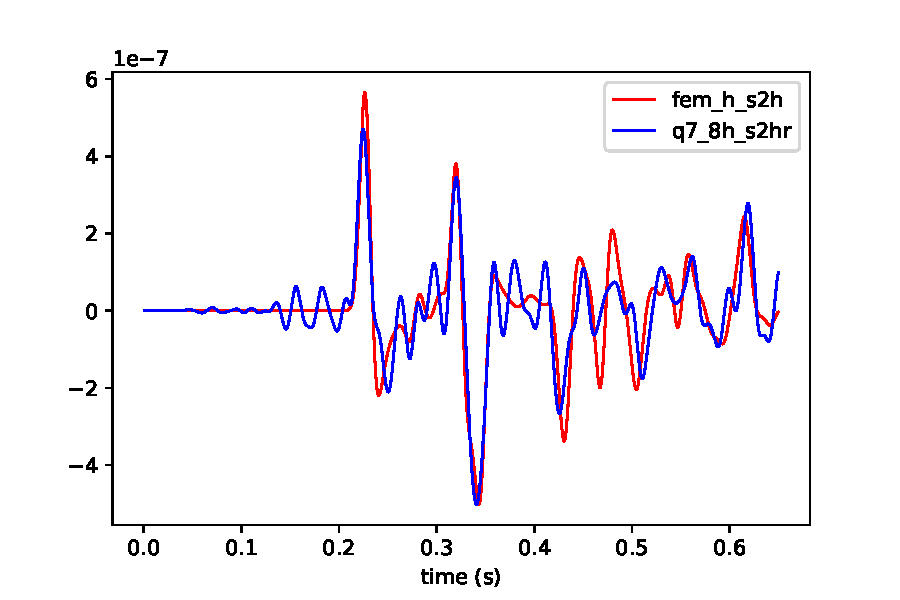
\includegraphics[width=8cm, height=6cm]{Thesis_Edith/figures/topo/topo_waves/gfem7_topo_tr75.pdf}
	\caption{Topographic model: Seismograms of the reference solution and a GFEM case with 7 wave plane directions in a coarse mesh of $8h$ for a receiver located at 580.3 in the horizontal coordinate.}
	\label{fig:4.1}
\end{figure}

A similar effect on the accuracy of the solution is produced by the mesh - source size relationship as explored in case 1. In this case, I showed that the source radius needs to be at least equal to the mesh size to improve the accuracy of the GFEM simulations. Nevertheless, a way to circumvent this requirement  and  implement a smaller source size than the background mesh is to perform local mesh refinement around the source. Evidently, this additional refinement increases the overall DOFs of the sytem, but as results show (See for instance Figures \ref{fig:3.13} and  \ref{fig:3.36}), this effect in the simulation time is minimal, with the additional benefit of further reducing the simulation errors.  

In this work, I have also shown important advantages of the GFEM  as in the implementation of flexible meshing with conforming and non-conforming local mesh refinement. These features have been exploited not only when performing local refinement around the source to implement smaller source sizes but also in the meshing of complex boundaries as in cases 3 and 4, in which a karst structure and topographic relief are included in the geological models. In case 3, the scattering model shows the benefit of including the additional refinement around the karst inclusion to conform better to its boundary.  As shown in Figures \ref{fig:3.29} and \ref{fig:3.30}, this additional refinement improved the accuracy of reflections coming from the karst boundaries. In case 4, the topographic model, unstructured meshes make possible to generate boundary-conforming meshes along the the topographic relief. As discussed in the introduction, this is one of the most problematic issues when using finite difference methods, since finite difference does not allow in a straight forward manner to implement unstructured meshes with local refinement.

An aspect that is relevant for the computational efficiency of the simulations, but not explored in this work, is related to appropriate techniques for solving the matrix equation at every time step. To solve this type of equation is, in general terms, very costly for continuous FEM approaches, including GFEM, since it involves the inversion of commonly large, albeit sparse, mass matrices \cite{DeBasabe2009}. For this work, I used a direct multifrontal solver based on the LU factorization since this method can handle sparse and rank-deficient matrices as they may occur in the GFEM approach. However it is known that the efficiency of these type of solvers degrades for large systems. Nevertheless, recent developments in direct solver algorithms are providing more efficient techniques as for the case of direct solvers with QR factorization as applied in \cite{Bogiatzis2016}. A more common and effective approach to handle large systems is to diagonalize the  mass matrix by applying mass lumping techniques \cite{JENSEN1996} as a preconditioning step.  Yet, a completely different methodology that can provide a good improvement in efficiency is to implement a discontinuous Galerkin (DG) FEM-GFEM formulation, instead of a continuous one,  as suggested in \cite{Hiptmair2016}. An important advantage of the DG formulation is that it produces a block diagonal mass matrix \cite{Grote2006} that is more amenable to invert, saving computational cost. 






